%
% Sección de comparación de desempeño,
% presentación de TT 1.
%
% Proyecto Lovelace.
%

\subsection{Resultados}

\begin{frame}{Resultados}{Comparaciones de desempeño}
  \only<1>
  {
    Las pruebas mostradas a continuación se realizaron en una computadora
    Toshiba S55-B5289 con las siguientes especificaciones:
    \begin{itemize}
      \item Procesador Intel Core i7-4710HQ.
      \begin{itemize}
        \item 6M caché, hasta 3.50GHz.
        \item 8 núcleos.
      \end{itemize}
      \item 8GB de RAM.
      \item En los casos pertinentes, se utilizó AES-NI\footnotemark.
      \item Se utilizó el compilador GCC versión 7.3.1.
    \end{itemize}
    \footnotetext{
      \textit{Intel Advanced Encryption Standard New Instructions}.
    }
  }
  \only<2>
  {
    {\small
      \begin{table}
        \begin{center}
          \begin{tabular}{c|c|c|}
            \cline{2-3}
            & Tokenización & Detokenización \\
            \hline
            \multicolumn{1}{|c|}{BPS}
              & 359.088   $\mu$s & 357.620 $\mu$s   \\\hline
            \multicolumn{1}{|c|}{FFX}
              & 274.905   $\mu$s & 275.147 $\mu$s   \\\hline

            \multicolumn{1}{|c|}{TKR}
              & 74.424  $m$s & 669.203 $\mu$s   \\\hline
            \multicolumn{1}{|c|}{AHR}
              & 70.041  $m$s & 719.729 $\mu$s   \\\hline
            \multicolumn{1}{|c|}{DRBG}
              & 75.247  $m$s & 696.643 $\mu$s  \\\hline
          \end{tabular}

          \caption{Comparación de tiempos de tokenización.}
          \label{tabla:tiempos_tokenizacion}
        \end{center}
      \end{table}
    }
  }

  \only<3>
  {
    \begin{figure}[H]
      \begin{center}
        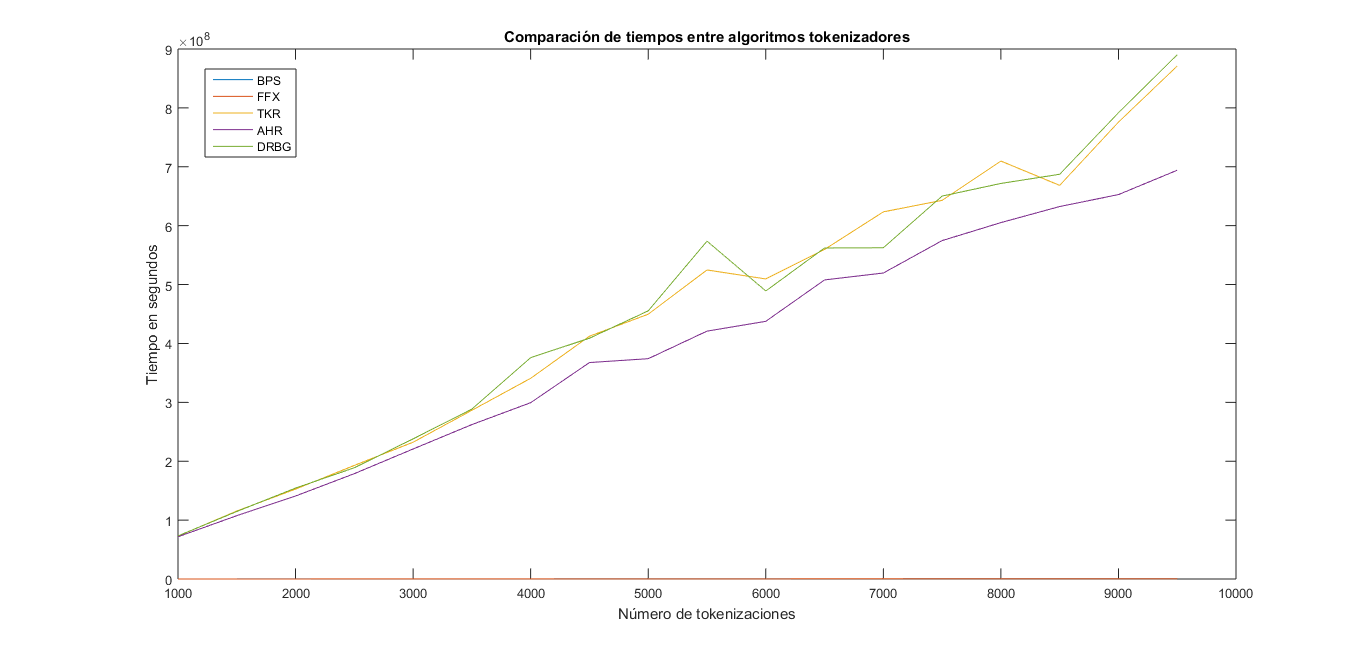
\includegraphics[width=1.0\linewidth]
          {../../../diagramas_comunes/desempenio/tok_todos.png}
        \caption{Tiempos de tokenización generales.}
      \end{center}
    \end{figure}
  }

  \only<4>
  {
    \begin{figure}[H]
      \begin{center}
        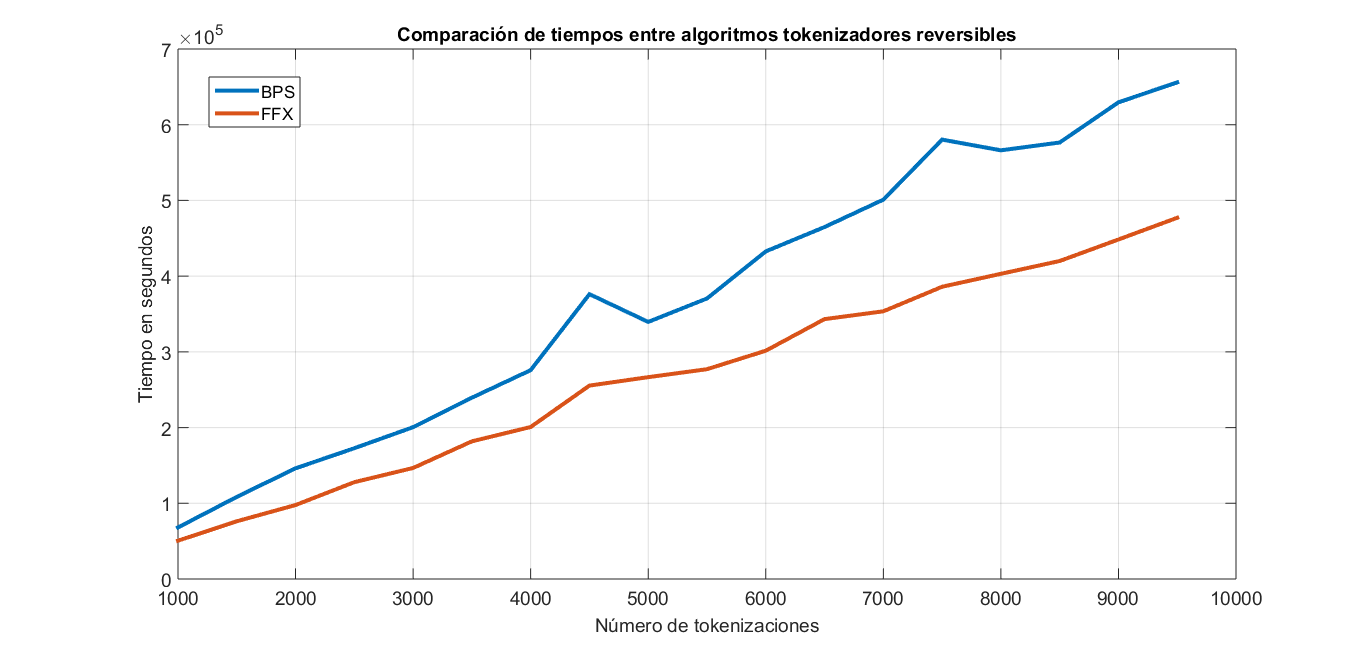
\includegraphics[width=1.0\linewidth]
          {../../../diagramas_comunes/desempenio/tok_rev.png}
        \caption{Tiempos de tokenización de reversibles.}
      \end{center}
    \end{figure}
  }

  \only<5>
  {
    \begin{figure}[H]
      \begin{center}
        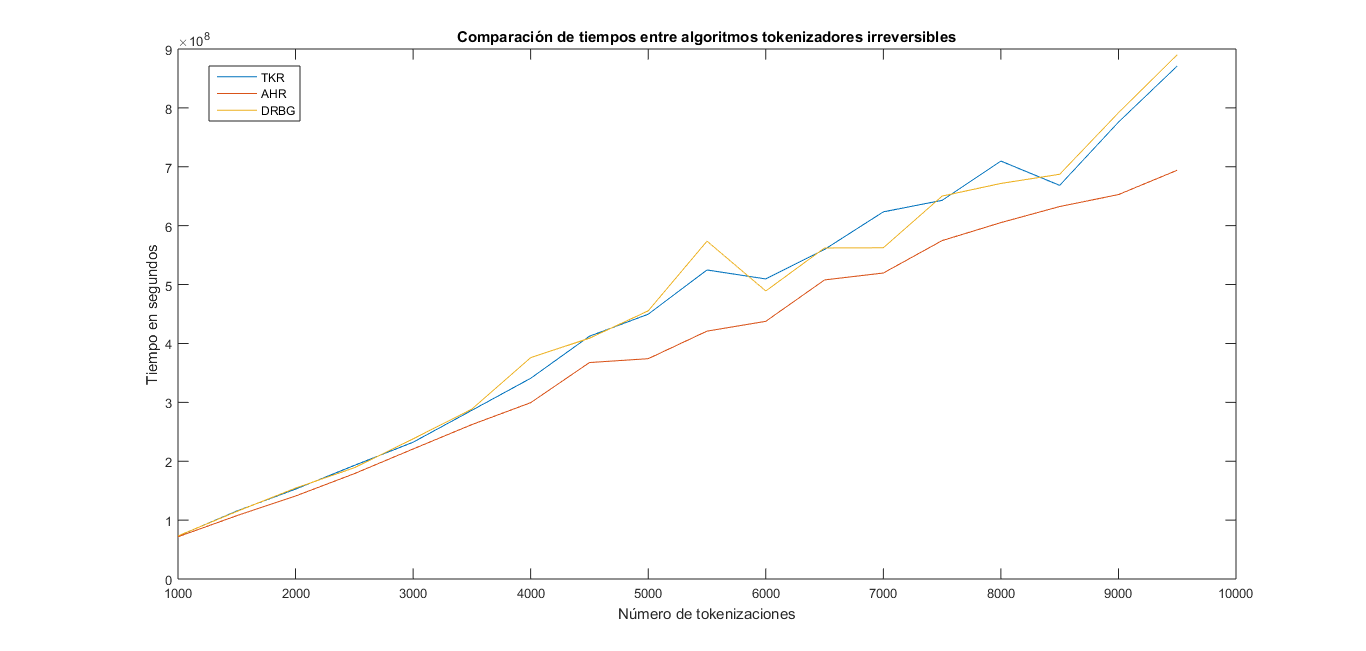
\includegraphics[width=1.0\linewidth]
          {../../../diagramas_comunes/desempenio/tok_irrev.png}
        \caption{Tiempos de tokenización de irreversibles.}
      \end{center}
    \end{figure}
  }

  \note
  {
    Los tiempos de los reversibles son mucho más cortos.

    Las gráficas muestran solo los procesos de tokenización: con la
    detokenización pasan cosas bastante similares.
  }

\end{frame}

\begin{frame}{Resultados}{Pruebas de aleatoriedad}

  En~\cite{nist_pruebas} el NIST describe un conjunto de 15 pruebas
  estadísticas que sirven para determinar la aleatoriedad de un generador
  pseudoaleatorio.

  Para cada instancia de los generadores implementados se ejecutó el conjunto
  de pruebas 20 veces, cada una con medio millón de bits (un total de veinte
  millones).

\end{frame}

\begin{frame}{Resultados}{Pruebas de aleatoriedad}

  Resultados de las pruebas de aleatoriedad para generadores basados en
  funciones hash y cifrados por bloque:

    \begin{table}
      \begin{center}
        \begin{tabular}{|c|c|c|}
          \hline
          Nivel de seguridad &
          Funciones hash &
          Cifrados por bloque \\\hline
          112 bits & 14 de 15 & 15 de 15 \\\hline
          128 bits & 15 de 15 & 15 de 15 \\\hline
          192 bits & 14 de 15 & 15 de 15 \\\hline
          256 bits & 15 de 15 & 15 de 15 \\\hline
        \end{tabular}
        \caption{Resultados de las pruebas de aleatoriedad.}
      \end{center}
    \end{table}

  \note
  {
    Estrictamente hablando, el generador basado en una función hash no es
    totalmente aleatorio, dado que falló en un par de pruebas. Sin embargo,
    el número de veces que se ejecutó el conjunto de pruebas (veinte) es
    un número relativamente pequeño (en comparación con lo recomendado por
    el NIST); esto por los recursos de cómputo que las pruebas exigen.
  }

\end{frame}
